% file: k-sorting.tex

\documentclass[tikz]{standalone}
\usetikzlibrary{decorations.pathreplacing, positioning, arrows.meta, shapes.multipart}

\begin{document}
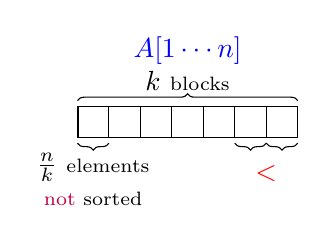
\begin{tikzpicture}[KS/.style = {rectangle split, rectangle split parts = 7, rectangle split horizontal, 
  	draw, anchor = center}]
  \node[KS] (ks) {};

  \draw[decoration = {brace, raise = 2pt}, decorate] (ks.north west) -- node[above = 2pt, align = center] 
	{\textcolor{blue}{$A[1 \cdots n]$} \\ $k$ {\scriptsize blocks}} (ks.north east);
  \draw[decoration = {brace, mirror, raise = 2pt}, decorate] (ks.south west) -- node[below = 2pt, align = center] 
	{$\frac{n}{k}$ {\scriptsize elements} \\ {\scriptsize \textcolor{purple}{not} sorted}} (ks.one split south);

  \draw[decoration = {brace, mirror, raise = 2pt}, decorate] (ks.five split south) -- node[below = 2pt] (b6)
	{} (ks.six split south);
  \draw[decoration = {brace, mirror, raise = 2pt}, decorate] (ks.six split south) -- node[below = 2pt] (b7)
	{} (ks.south east);
  \path[] (b6) -- node[below = 1pt] {\textcolor{red}{$<$}} (b7);
\end{tikzpicture}
\end{document}
